% EPL master thesis covers template
\documentclass{eplmastersthesis}
\usepackage{float}

% Please fill in the following boxes
% Title of the thesis
\title{Integrated mini-cloud of RaspberryPIs for distributed systems training}

% Subtitle - remove this line if not applicable
\subtitle{The Splay Project}

% Name of the student author(s)
\author{Rémy \textsc{Voet}}
\secondauthor{Samuel \textsc{Monroe}}		% remove if not applicable
%\thirdauthor{Firstname \textsc{Lastname}}			% remove if not applicable

% Official title of the master degree (copy/paste from list below)
% Master [120] in Biomedical Engineering
% Master [120] in Chemical and Materials Engineering
% Master [120] in Civil Engineering
% Master [120] in Computer Science
% Master [120] in Computer Science and Engineering
% Master [120] in Cybersecurity
% Master [120] in Data Sciences Engineering
% Master [120] in Data Science: Information technology
% Master [120] in Electrical Engineering
% Master [120] in Electro-mechanical Engineering
% Master [120] in Mathematical Engineering
% Master [120] in Mechanical Engineering
% Master [120] in Physical Engineering
% Master [60] in Computer Science
% Specialised master in nanotechnologies
% Specialised master in nuclear engineering
\degreetitle{Master [120] in Computer Science}

% Name of the supervisor(s)
\supervisor{Étienne \textsc{Rivière}}
%\secondsupervisor{Firstname \textsc{Lastname}}		% remove if not applicable
%\thirdsupervisor{Firstname \textsc{Lastname}}		% remove if not applicable

% Name of the reader(s)
\readerone{Firstname \textsc{Lastname}}
\readertwo{Firstname \textsc{Lastname}}			% remove if not applicable
\readerthree{Firstname \textsc{Lastname}}			% remove if not applicable
%\readerfour{Firstname \textsc{Lastname}}			% remove if not applicable
%\readerfive{Firstname \textsc{Lastname}}			% remove if not applicable

% Academic year (update if necessary)
\years{2018--2019}

% Document
\begin{document}
  % Front cover page
  \maketitle

  \chapter*{Abstract}

  \chapter*{Acknowledgements}

  \tableofcontents

  \chapter{Introduction}

    \section{Context and Motivations}

      The process of learning distributed systems and algorithms is usually
      undermined by the difficulty of being able for one to test and apply
      what he learns.\\
      Indeed, in order to run a distributed algorithm and observe the result, a
      collection of machines running the algorithm is needed. Besides that,
      one would like to be able to change the conditions in which the algorithm
      is run, for example by provoking faulty nodes, or inducing network
      perturbations among the system, as distributed algorithms are designed to
      adapt to these conditions. These needs make it really cumbersome
      for students to setup a testing environment emulating realistic
      conditions for learning purposes.

    \section{About the Splay Project}

      Discussion about what was available when we started the rework of
      the Splay project.

    \section{Objectives}

      Detailed objectives of the system and our update.

    \section{Features}

      The features available to the users (distributed algorithm editor on the
      web-page, fault injection, topology).

      \subsection{Scenarios}

        Scenarios of usage making use of the different features available.


  \chapter{Software Architecture}

    % About all the Splay software parts.
    

    \section{Legacy Architecture}

      How Splay was design.

      % Figure of the old architecture, TODO : remake with technologies used
      \begin{figure}[H]
        \centering
        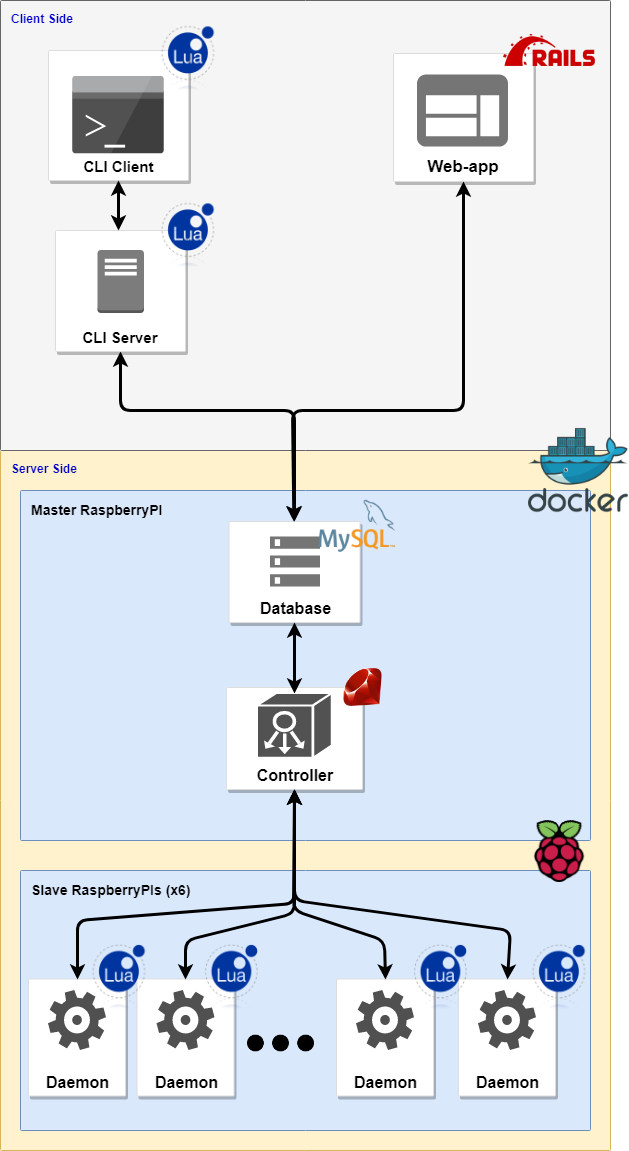
\includegraphics[scale=0.6]{figures/prev_arch.png}
        \caption{\label{prev_arch} Previous Splay Architecture}
      \end{figure}


    \section{Renewed Architecture}

      How we changed Splay.
      \begin{figure}[H]
        \centering
        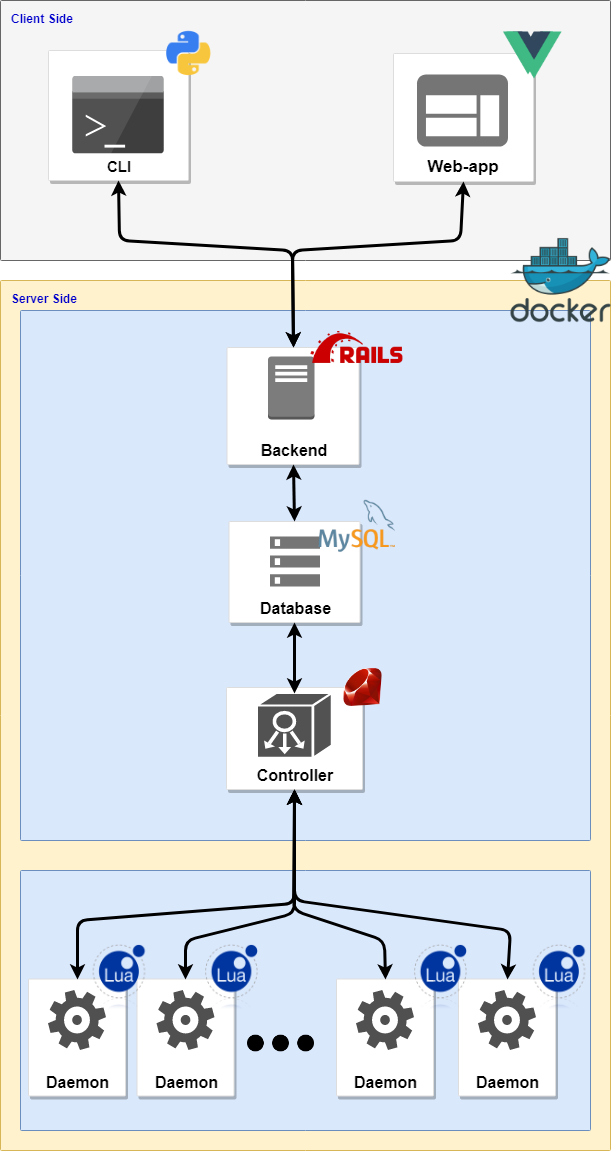
\includegraphics[scale=0.105]{figures/new_arch.png}
        \caption{\label{new_arch} New Splay Architecture}
      \end{figure}

  \chapter{Hardware Architecture}

    About the Rasp cluster.

  \chapter{Development Methodology}

    Before talking about the implementation details, we talk about how we actually
    organized ourselves in order to develop the application and ensure quality
    through the Gitflow system and using code reviews along our pull requests
    in order to maintain a global knowledge of the system, even if we had to work
    on different parts of the system.

  \chapter{Implementation}

    Implementation details  (following a story-telling approach?).

    \section{Technology choices}

      Details about the different technologies used.

    \section{Github Repository Cleaning}

      First step was to clean the github repo

    \section{Centralization of Splay's Backend}

      How we moved the old rails app and cli server to a single backend
      to serve any app wanting to connect with Splay.

    \section{A new front-end application}

      As backend was available, development of a VueJS SPA.

    \section{Rework of the CLI to use new Backend}

      All the Command line interface has been redone in Python more clearly and concise.

    \section{Topology creation through Javascript Interface}

    \section{Fault injection}
    
  \chapter{Testing and Validation}

    We wanted to reach 100\% LOC testing with feature testing, unit testing,
    and testing the whole system with rock solid test suite, must explain this.



  \chapter{Conclusion}




  % Back cover page
  \backcoverpage

\end{document}
